\chapter{Abenteuer vorbereiten}\label{Ch:AbenteuerVorbereiten}
\lettrine[lraise=0.1]{F}{ür} das Erschaffen von guten Geschichten gibt es leider kein Patentrezept. Insbesondere das W"ortchen `gut' stellt ein h"aufiges Problem dar. Im letzten Kapitel wurden bereits verschiedene Abenteuer-Typen und Ideen für den Inhalt vorgestellt. In diesem Abschnitt wird \emph{eine} (von unzähligen) Methode zur Erschaffung von auf die Charaktere zugeschnittenen Geschichten vorgestellt. Mit ein wenig Phantasie sollte es damit gelingen, den Einstieg f"ur eine Kampagne \StoryDSA zu finden.







\section{Verschiedene Arten von Abenteuern}
Abenteuer unterscheiden sich voneinander, sowohl inhaltlich als auch von der Form her. Obwohl \StoryDSA dem Spielleiter für das Nachspielen einer Geschichte mit mehr oder weniger festem Verlauf recht umfangreiche Kompetenzen einräumt, wird es auch in solchen Situationen immer wieder vorkommen, dass der Spielleiter sich mit einer unvorhergesehenen Idee konfrontiert sieht und improvisieren muss. In solchen Fällen machen starre Abenteuerformen mehr Probleme als andere, bei denen die Improvisation von vorne herein geplant ist.

\subsection{Inhaltliche Aufteilung}
Die Charaktere in \StoryDSA sind anfangs unbekannte Jung-Abenteurer (mit jung ist hier das Dienstalter, nicht das tatsächliche Alter gemeint), die sich Ruhm und Ehre erarbeiten und so in Aventuren zu bekannten Helden aufsteigen. Daher sollten die meisten Abenteuer auch Heldenhaftigkeit zulassen -- dazu gehört vor allem, dass die Welt von den guten Taten der Charaktere auch erfahren wird und nicht, dass die Charaktere im stillen Kämmerlein gefährliche Dinge tun, die die Welt nicht interessiert oder mitbekommt.

Folgende Inhalte decken wahrscheinlich den größten Teil der möglichen Abenteuer ab. Dabei sind die einzelnen Punkte nicht streng voneinander getrennt; viele Geschichten, fallen in mehrere der aufgezählten Kategorien. Zudem ist in der Aufzählung immer von einem SLC die Rede; dies können natürlich auch jeweils mehrere sein.
\begin{description}
\item[Auftrag:] Ein SLC ist auf fremde Hilfe angewiesen und beauftragen die Helden, etwas zu machen. Dabei handelt es sich natürlich üblicherweise um heldenhafte Dinge, wie z.\,B. die Aufklärung eines Mordes oder die Bewachung einer Karawane.

\item[Notfall:] Ein SLC steckt in einer problematischen Lage. Die Helden werden auf den Missstand aufmerksam und versuchen, das Problem aus der Welt zu schaffen. Typische Beispiele sind eine Entführung, ein tyrannischer Baron oder ein unschuldig auf seine Todesstrafe wartender Adelsspross. Eventuell ist das Beseitigen des Problem auch relativ einfach und das eigentliche Abenteuer dreht sich um die Aufklärung bzw. das Auffinden des Verursachers.

Eine Verschärfung dieser letzten Idee stellt eine Intrigen-Situation dar, in der die SCs vom wahren Verursacher für die missliche Lage verantwortlich gemacht werden. So könnten die Helden auf einmal des Mordes angeklagt werden.

\item[Konkurrenz:] Die Charaktere stehen in Konkurrenz zu einem SLC. Sie wollen dasselbe Ziel erreichen, müssen aber schneller, besser und eben auch heldenhafter sein als ihr Konkurrent. Bei diesem Ziel ist es wichtig, dass es keine Friede-Freude-Eierkuchen-für-alle-Lösung gibt, d.\,h. wenn der Konkurrent gewinnt, haben die Helden ihr Ziel eben nicht erreicht. Das Gewinnen eines Turniers, die schnellere Umrundung der Welt oder die Jagd nach einem Schatz sind drei der möglichen Szenarien.

\item[Dingliches:] Die Abenteurer erfahren von einer möglichen Großtat, die noch niemand zuvor begangen hat oder kommen in eine Situation, die sie heldenhaft meistern müssen: Beispielsweise bekommen sie eine Schatzkarte, wollen unbekannte Lande kartieren oder stranden an einer gefährlichen Insel auf der sie ihr Überleben sichern müssen, bis sie entkommen können. Wie auch immer, es gibt eine Heldentat auf der Welt, die die Charaktere aus eigener Motivation heraus erledigen wollen (und sei es nur zu überleben). Bei rein Dinglichen Abenteuern gibt es keine für die Geschichte SLCs außer einfachen Gegnern, Monstern und andere Gefahren, die überwunden werden müssen.

\item[Zwischen den Fronten:] Mehrere SLC-Gruppen haben konkurrierende Interessen und streiten darum. Die SCs geraten irgendwie zwischen die Fronten und werden mit in die Sache hineingezogen. Sie können sich für eine Seite entscheiden oder versuchen zu schlichten. Hineingezogen werden können sie aus eigenem Interesse (so stellen die Abenteurer eventuell eine weitere Gruppierung) oder weil eine Seite auf die Idee kommt, sie für ihre Zwecke einzusetzen.

\item[Neider:] Es gibt einen SLC, der etwas will, was die Charaktere schon haben. Dabei kann es sich um eine gute Position handeln oder auch um einen Gegenstand. Damit aus der Abwehr des Neiders ein heldenhaftes Abenteuer wird, sollte die Beseitigung des Neiders nicht den Zorn der anderen SLCs nach sich ziehen.
\end{description}

Bei all diesen Ideen darf der Spielleiter trotz alledem die Heldenhaftigkeit nicht aus den Augen verlieren. Wie oben schon angedeutet, sollte die Welt (meistens) eine glaubwürdige Möglichkeit haben, von den Taten der angehenden Helden zu erfahren.

Andere Geschichten, die wahrscheinlich auch Spaß beim Spiel bereiten, die aber nicht gut von \StoryDSA unterstützt werden, handeln beispielsweise von den Liebesaffähren einer verzweifelten Hausfrau, von Richterin Salesa und ihren Verhandlungen oder den besonderen Fällen von Heiler Gregorius.

\subsection{Formale Aufteilung}
Im Gegensatz zum Inhalt ist der Aufbau des Abenteuers entscheidend dafür, wie frei die Spieler ihre Charaktere ausspielen können. Natürlich sind Form und Inhalt teilweise miteinander verknüpft, trotzdem ist die Art und Weise der Vorbereitung entscheidend dafür, wie einfach oder schwierig es für den Spielleiter ist, sich während des Spiel auf unvorhergesehene Ideen einzustellen. Die folgende Aufzählung gibt Hinweise und Tipps, welche Formen möglich sind und wo die Vor- und Nachteile liegen.

\begin{description}
\item[Situationsbasiertes Abenteuer]
    Der Spielleiter bereitet Situationen vor, die nacheinander gespielt werden.
    Diese Stationen können hinderlich oder für den weiteren Verlauf hilfreich
    sein. Auf eine Situation können je nach Ausgang verschiedene andere folgen,
    es kann Kreise geben, usw. Man kann situationsbasierte Abenteuer gut in
    einem Ablaufdiagramm mit Pfeilen für die möglichen Übergänge darstellen.

    Gerade situationsbasierte Abenteuer mit jeweils nur einer Nachfolgestation,
    auch \DEF{lineare Abenteuer}\index{Abenteuer!linear} genannt, werden oft als
    einengend empfunden.
    Es kann schnell passieren, dass die Spieler auf Ideen kommen, die der SL in
    seiner Vorbereitung nicht vorgesehen hat und dass die Situationen dann
    nicht mehr sauber aneinander passen. Einmal ausgebrochen kann es schwierig
    oder sogar unmöglich sein, wieder zum Plan zurückzufinden. Hier ist
    eventuell großes Improvisationstalent gefragt.

    Andererseits sind situationsbasierte Abenteuer einfach zu leiten, wenn die
    Spieler im Rahmen bleiben. Die Situationen können vorbereitet werden; der
    Spielleiter muss nur wenig Entscheidungen spontan treffen.

\item[Ortsbasiertes Abenteuer]
    Der Spielleiter bereitet Stationen wie in einem situationsbasierten
    Abenteuer vor, die allerdings nicht in einer logischen Struktur zueinandern
    sondern auf einem Plan angeordnet werden. Die Spieler steuern ihre
    Charaktere über den Plan und spielen die Situationen an denen sie
    vorbeikommen.

    Auch bei ortsbasierten Abenteuern kann es zur Gängelung kommen, wenn
    die SCs versuchen, aus der vorgegebenen Karte auszubrechen. Dies kann durch
    geschickten Einsatz von Sicherungsmaßnahmen oder durch gute Motivation der
    SCs verhindert werden.

    Auch ortsbasierte Abenteuer sind recht einfach zu leiten, da die
    Situationen, in denen relevante Dinge passieren, gut vorzubereiten sind.
    Alleine die Reihenfolge ist nicht klar, weswegen die einzelnen Situationen
    in der hier angegebenen Reinform nur schwer miteinander in Verbindung
    gebracht werden können. Damit können solche Abenteuer leich aufgesetzt
    wirken.

\item[Ereignisbasiertes Abenteuer]
    Der Spielleiter bereitet Ereignisse vor, die auf einem Plan angeordnet
    werden und zu vorgegebenen Zeitpunkten eintreten. Meist gibt es
    Abhängigkeiten und Beziehungen unter den Ereignissen. Die Spieler
    müssen bestimmte Ereignisse verhindern oder verändern. 

    Bei dieser Art von Abenteuer ist die Freiheit der Spieler relativ groß. 
    Das eigentliche Problem dabei ist es, dass Ereignisse eintreten und die Spieler
    dies nicht mitbekommen, weil die Charaktere nicht vor Ort sind.
    Die größte Schwierigkeit ist es also für den
    Spielleiter, den \emph{Spielern} klar zu machen, wann und wo das nächste Ereignis
    stattfindet, damit die Charaktere auch daran teilnehmen können und das
    Spiel nicht langweilig wird. In der Vorbereitung sollte daher darauf viel
    Wert gelegt werden.

\item[Charakterbasiertes Abenteuer]
    Der Spielleiter bereitet SLCs vor, die alle persönliche Ziele haben.  Diese
    Ziele sind meistens widersprüchlich, eventuell betreffen diese Widersprüche
    auch direkt die SCs. Die Spieler müssen die Konflikte unter den SLCs lösen.

    Charakterbasierten Abenteuern beinhalten wahrscheinlich die größte 
    Spieler-Freiheit, denn der Spielleiter muss ja nur die Wünsche und Ziele
    der SLCs darstellen. Dabei ist diese Art von Abenteuer leider auch am
    schwierigsten zu leiten,
    denn der SL muss seine Charaktere glaubhaft und unterscheidbar darstellen.
    Daher ist es für den Spielleiter wichtig, sich über Motivationen,
    Handlungsgrenzen und Charaktereigenschaften wirklich im klaren zu sein.
    Auch ein Klischee oder ein klares Charakterkonzept helfen bei der
    Darstellung ungemein.
\end{description}

Diese Grund-Typen können natürlich miteinander kombiniert werden. Ein
Spielleiter kann in einem ortsbasierten Abenteuer SLCs mit widersprüchlichen
Zielen unterbringen, er kann in einem charakterbasierten Abenteuer Ereignisse
zu bestimmten Zeiten eintreten lassen usw. Tatsächlich wird es kaum Abenteuer
geben, die eine der obigen Typen in Reinform darstellt. Bekannte Beispiele für solche
Mischformen sind:

\begin{description}
\item[Der Dungeoncrawl]
    Sicherlich eine der ältesten Abenteuerformen. Im Wesentlichen ist ein
    Dungeoncrawl ein ortsbasiertes Abenteuer, in dem die Charaktere durch die
    Wände am Ausbrechen aus dem Plot gehindert werden. Durch die
    Ganganordnungen können die Charaktere auch gezwungen werden, Stationen in
    bestimmten Reihenfolgen zu durchlaufen, was einem solchen Abenteuer
    situationsbasierte Elemente hinzufügt. Auch werden gerne Ereignisse oder
    Charaktere mit bestimmten Motivationen eingestreut, um den Dungeon weniger
    statisch zu gestalten.

\item[Der Shadowrun]
    Die Charaktere bekommen einen Auftrag. Sie können zunächst im Stil eines
    situationsbasierten Abenteuers an einige Informationen gelangen und sich
    vorbereiten. Danach folgt ein ortsbasiertes (oder evtl. ein
    situationsbasiertes) Abenteuer eventuell vermischt mit ein paar
    Ereignissen, ähnlich zu einem Dungeoncrawl.

\item[Die Ermittlung]
    Eine Ermittlung besteht aus Stationen mit Hinweisen, widersprüchliche SLCs
    und Ereignissen, die auf einem Plan angeordnet werden. Die Spieler müssen
    Informationen sammeln, die sie benötigen, um ein bestimmtes Ziel zu
    erreichen (z.B. den Mörder überführen). Eine Ermittlung findet meist an
    einem eingegrenzten Ort statt (z.B. eine Ortschaft, ein großes Haus oder
    ein Gutshof).

\item[Die Schnizeljagd]
    Der Spielleiter bereitet Stationen, SLCs und Ereignisse vor, die jeweils
    Hinweise liefern, wo es weitergeht. Dadurch hat eine Schnitzeljagd oft den
    Charakter eines linearen Abenteuers, wobei die einzelnen Stationen
    recht aufwändig aufgebaut sein können. Das Abenteuer endet, wenn die
    Charaktere ein bestimmtes Ziel erreicht haben (z.B. einen Schatz finden).
    Eine Schnitzeljagd kann über große räumliche Entfernungen verlaufen.

\item[Episodenhaftes Abenteuer]
    Der Spielleiter bereitet Episoden vor, von denen jedes einzelne wie eines
    der oben vorgestellten Abenteuer-Typen aufgebaut ist. Die Episoden werden
    dann in einer bestimmten Reihenfolge durchlaufen und sind inhaltlich eng
    miteinander verknüpft. Es kann sehr breite oder auch sehr schmale Übergänge
    zwischen den einzelnen Teilen geben. Eventuell können auch ganze Abschitte
    übersprungen werden -- das ist aber selten, denn die Vorbereitung ist für
    jeden Abschnitt recht aufwändig. Die einzelnen Kapitel sind normalerweise
    inhaltlich nicht in sich abgeschlossen. Man kann daher eine Schnitzeljagd
    als Unterform der episodenhaften Abenteuer auffassen.

\item[Die Kampagne]
    Eine Kampagne ist eine Folge von Abenteuern, die aufeinander aufbauen aber
    jeweils inhaltlich abgeschlossen sind. Oft bereitet der Spielleiter immer
    nur das nächste Abenteuer, basierend auf dem bisherigen Spielverlauf, vor
    und weiß selber höchstens grob, wie es danach weitergehen wird. Teilweise
    können Kampagnen auch als Abenteuermodule gekauft werden und sind dann
    natürlich von langer Hand geplant. Dann ähneln solche Kampagnen eher
    besonders langen episodenhaften Abenteuern.
\end{description}



\section{Werkzeuge zur Vorbereitung}
Nachdem jetzt verschiedene Arten von Geschichten, die sich für \StoryDSA eignen, bekannt sind, werden in diesem Abschnitt ein paar formalisierte Methoden zum übersichtlichen Notieren von Abenteuern vorgestellt. Für selbst erdachte Abenteuer, aber auch für Kaufabenteuer, stellen solche Werkzeuge gute Hilfen zur Vorbereitung dar.


\subsection{Der Kern des Abenteuers}\label{subsec:DerKernDesAbenteuers}
Für die Spieler ist es im Normalfall befriedigend, wenn sie erkennen können, wann ein Abenteuer abgeschlossen ist. Am besten ist es natürlich, wenn ihre Charaktere gewonnen haben; wichtiger ist jedoch das klar definierte Ende. Um eine solche Trennung zu erreichen, ist es günstig, die Idee der einzelnen Teile in ein oder maximal zwei kurzen Sätzen beschreiben zu können. Dabei ist das Verb besonders wichtig, denn das ist es ja, was \emph{zu tun} ist. Kommt einem für das Abenteuer kein charakteristisches Verb in den Sinn, so ist es wahrscheinlich zu unscharf umrissen und sollte nochmals überdacht werden.

\begin{beispiel}
\paragraph{Beispiele:} Ein paar gut umrissene Geschichten:
\begin{itemize}
\item Stellen des Assasinen, der den Baron getötet hat
\item Das rondrageweihte Schwert `Donnerbringer' finden
\item Aufklären der Ork-Überfälle in der Gegend um Donnerbach und Schlichtung des Streites zwischen Schmiede- und der Flusshändler-Gilde
\end{itemize}

In allen diesen Fällen ist genau klar, worum es geht und wann das Abenteuer beendet ist.
\end{beispiel}

Gerade auch bei Kaufabenteuern sollte sich der Spielleiter darüber Gedanken machen, was der Kern des Abenteuers ist. Beispielsweise sind viele in Kaufabenteuern beschriebene Szenen nur Beiwerk und könnten genauso gut weggelassen oder anders gespielt werden. Ist sich der Spielleiter des Kerns des Abenteuers bewusst, so kann er leichter entscheiden, was er für ein höheres Tempo überspringen kann oder in welchen Szenen die Spieler ihre Charaktere auch gegen den Vorschlag des Autors handeln lassen kann. 



\subsection{Flussdiagramme}
Ein hervorragendes Werkzeug f"ur die Planung von situationsbasierten Abenteuern (mit allen Vor- und Nachteilen, die ein solches Abenteuer mit sich bringt) ist die Erstellung eines \DEF{Flussdiagramms}\index{Flussdiagramm}. Dabei sollte sich der Spielleiter nochmal die Struktur von SL-Erz"ahlphasen, Konflikten und freiem Spiel ins Ged"achtnis rufen. Diese drei Arten von Szenen k"onnen "uber verschiedene Formen gut dargestellt werden: Rechtecke f"ur SL-Erz"ahlphasen, Ovale f"ur freies Spiel und auf der Spitze stehende Rauten f"ur Nebenkonflikte; Hauptkonflikte bekommen ein Dreieck. Wenn es bei unterschiedliche Ausg"ange f"ur gewonnene bzw. verlorene Konflikte gibt, so k"onnen die verbindenden Pfeile einfahch mit $+$ oder $-$ gekennzeichent werden.

\begin{figure}
\centerline{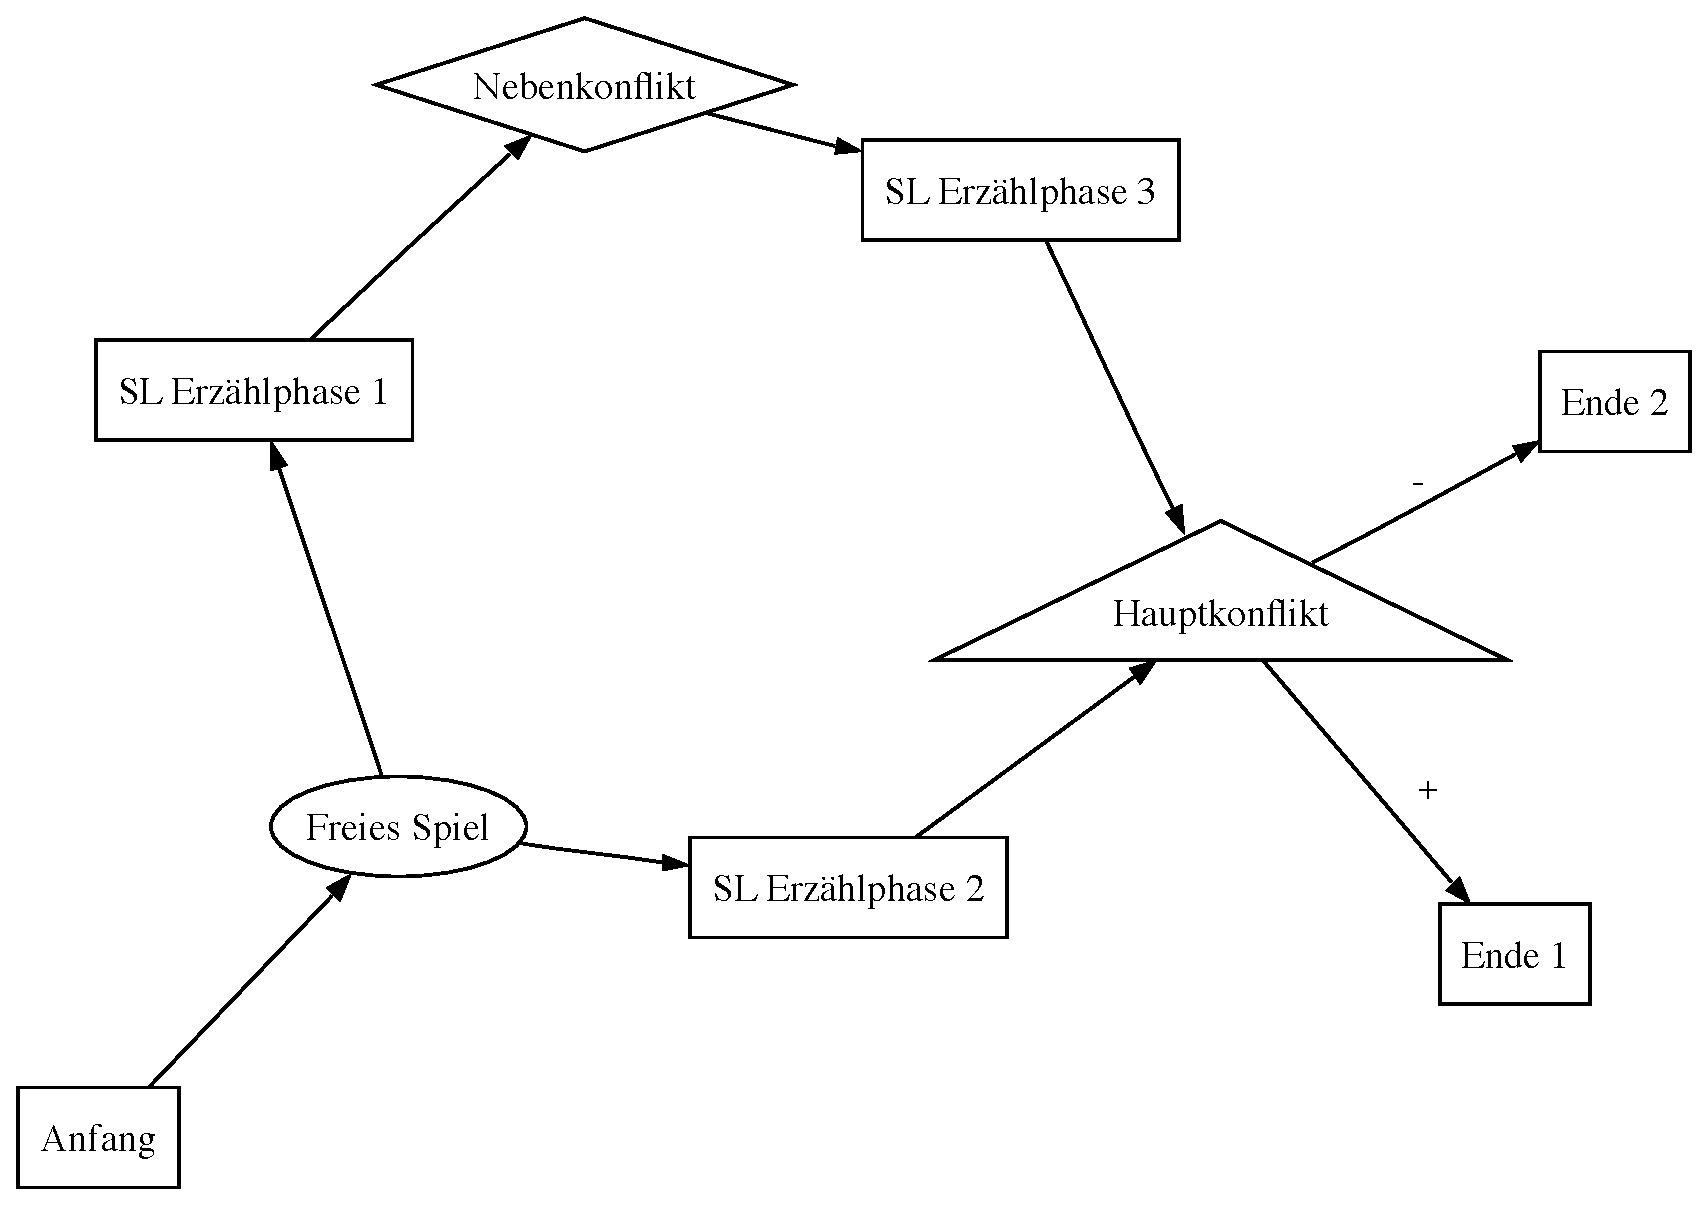
\includegraphics[width=0.95\textwidth]{pics/fluss1}}
\end{figure}

Fluss-Diagramme k"onnen auf verschiedene Arten benutzt werden: Ersten kann man mit ihnen, wie gerade angedeutet, den Verlauf des Abenteuers vorplanen. Zweitens k"onnen damit aber auch Handlungen von SLCs geplant werden. So k"onnten beispielsweise ein paar SLCs einen Einbruch geplant haben und die SCs versuchen, diesen zu entdecken. Legt der Spielleiter vorher einen Ablaufplan mit Zeiten f"ur den "Uberfall an, so kann er die Spieler im freien Spiel entscheiden lassen, wohin sie sich wann wenden wollen und dann entsprechend darauf reagieren.

\subsection{Karten}
\DEF{Karten}\index{Karte} eignen sich besonders für die Organisation von orts- und ereignisbasierten Abenteuern. Eine Landkarte, Stadtkarte oder Grundrisszeichnung hilft außerdem, sich den Ort besser vorstellen zu können. In solche Karten werden dann die Orte der Stationen und Ereignisse eingetragen.

Übergänge zwischen den einzelnen Stationen und Ereignisse werden dann im Spiel zu SL-Erzählphasen, Entscheidungen für das weitere Vorgehen werden im freien Spiel getroffen und das, was an wichtigen Dingen an den Stationen passiert, wird als Konflikte ausgetragen.

Karten sind oft nützliche Hilfsmittel, trotzdem sollte man es nicht mit ihnen übertreiben, da durch Karten auf immer eine Menge Freiheit verloren geht. So könnte die Grundrisszeichnung eines Hauses, das den Schauplatz für den großen Endkampf darstellt, die Spieler in ihren Erzählungen unnötig einschränken. Darüberhinaus ist die Erstellung einer Karte auch meist mit viel Arbeit für den Spielleiter verbunden -- und wenn eine Karte nicht unbedingt für einer orts- oder ereignisbasiertes Abenteuer benötigt wird, dann ist der Nutzen im Vergleich zum Aufwanf meist doch eher klein.

\subsection{Zeitplan}
In ereignisbasierten Abenteuern ist ein \DEF{Zeitplan}\index{Zeitplan} fast unverzichtbar und wesentlich wichtiger als eine Karte. Im Zeitplan sind alle Ereignisse aufgelistet, die vom Spielleiter vorbereitet sind. Oft hängen die Ereignisse auf gewisse Art und Weise zusammen, so dass sich bei genügend großer Komplexität für die Form des Zeitplans auch ein Flussdiagramm anbieten könnte. Der Weg durch diesen Zeitplan wird dann durch die Handlungen der Spielercharaktere festgelegt.

Im Gegensatz zum Flussdiagramm oben ist ein Zeitplan aber immer an die fortschreitende Zeit gekoppelt. Insbesondere wird man im Zeitplan üblicherweise nicht rückwärts gehen. Ausgehend von der Situation zu Beginn des Abenteuers verzweigen sich die Wege oder vereinigen sich wieder.

Aber auch für alle anderen Abenteuertypen sind Zeitpläne interessant. Es ist nützlich für den Spielleiter, eine \DEF{Eskalation}\index{Eskalation} der Situation in der Hinterhand zu haben, um die Charaktere (notfalls mit Gewalt) ins Abenteuer zu bringen. Dazu sollte der Spielleiter eine Folge von Ereignissen festlegen, die bestimmte Flaggen der Spielercharaktere und die Gefühle der Spieler (z.\,B. Hilfsbereitschaft, Kriegerehre, Moral) massiv ansprechen. Reagieren die Spieler nicht auf das Abenteuer, so kann der Spielleiter die Ereignisse der Eskalation eintreten lassen und so die Aufmerksamkeit auf das Abenteuer lenken. Der Zeitplan für eine Eskalation der Situation ist also normalerweise kein Zeitplan, der strikt eingehalten wird. Vielmehr ist es ein Notfallplan, der benutzt werden kann, um Langeweile am Spieltisch zu verhindern.




\subsection{Konfliktnetzte}
Bei einem Konfliktnetz geht es darum, Konflikte zwischen verschiedenen Gruppierungen und Charakteren graphisch übersichtlich darzustellen. Daher eignen sie sich besonders für charakterbasierte Abenteuer. Dazu werden f"ur alle beteiligten Gruppen gro"se Rechtecke auf ein Blatt gemalt, f"ur die Charaktere Ovale. Geh"ort ein bestimmter Charakter zu einer Gruppe, so werden die Charaktere in die Gruppen hineingezeichnet.

Desweiteren werden Charaktere und Gruppen untereinander mit Linien verkn"upft. Ans Ende werden Symbole gemalt, die dann f"ur eine bestimmte Grundhaltung steht. Dabei steht zur Verf"ugung:
\begin{itemize}
  \item ist freundlich gegen"uber (Kreis)
  \item ist feindlich gegen"uber (Dreieck)
  \item benutzt (Quadrat)
  \item kennt (Querstrich)
\end{itemize}

Es ist wichtig, dass im Konflikt-Netz nur Personen und Gruppen auftauchen, die f"ur die Geschichte relevant sind und auch miteinander verkn"upft sind. Es muss keine direkte Verbindung geben, jedoch sollte jeder Charakter "uber irgendwelche Wege mit jedem anderen Charakter verbunden sein. Ein Beispiel f"ur ein solches Konflikt-Netz ist auf Seite~\pageref{ConflictWeb1} zu finden.

Zusätzlich können diese Linien noch mit genaueren Informationen beschriftet werden, wie z.\,B. ``verheiratet'', ``Rivalen'', ``streiten um die Erbschaft'' usw.

\begin{figure}
\centerline{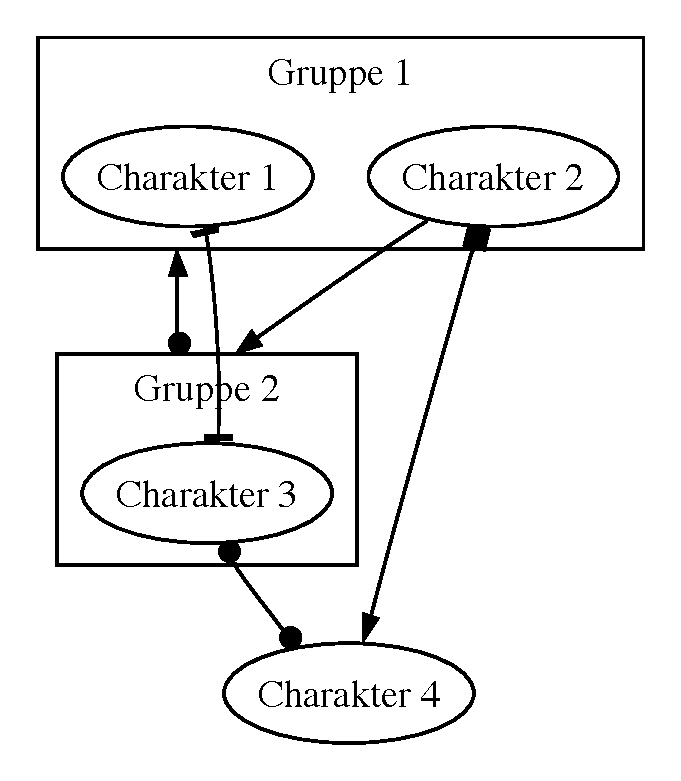
\includegraphics[height=0.55\textheight]{pics/web1}}

\paragraph{Erkl"arung des Schaubildes:} Charaktere~1 und~2 geh"oren zu Gruppe~1, Charakter~3 ist Mitglied von Gruppe~2 und Charakter~4 geh"ort keiner Gruppe an. Grunds"atzlich ist Gruppe~1 freundlich gegen"uber von Gruppe~2, Gruppe~2 aber feindlich gegen"uber Gruppe~1. Wahrscheinlich gibt Gruppe~2 vor, freundlich zu sein und Charakter~2 hat dies durchschaut, er ist n"amlich (als Ausnahme aller Charaktere aus Gruppe~1) feindlich gegen"uber Gruppe~2.

Charaktere~1 und 3 kennen sich zwar, haben aber sonst keine Meinung voneinander (d.\,h. sie wissen wahrscheinlich auch nichts von ihrer Gruppenzugeh"origkeit). Charakter~2 kann Charakter~4 nicht leiden, wird aber von diesem benutzt. Dagegen sind Charaktere~3 und 4 befreundet.

\label{ConflictWeb1}
\end{figure}








\section{Flaggen und Bangs}
Das wichtigste Hilfsmittel f"ur eine auf die Charaktere zugeschnittene Geschichte liefern die Charakterb"ogen und da insbesondere die Fragen an den Spieler und die Hintergrundgeschichte. Alles, was auf die Interessen der Spieler hindeutet, wird im folgenden als \DEF{Flagge}\index{Flagge} bezeichnet, also evtl. auch die Wahl der Profession, die Talente und die Vor- und Nachteile. Denn auch diese geben Aufschluss dar"uber, in welche Richtung die Geschichte gehen soll. So wird beispielsweise eine Gruppe Bannstrahler kaum stimmig in eine Geschichte verwickelt werden k"onnen, in der sie in einer heimlichen Nacht-und-Nebel-Aktion mit magischen Hilfsmitteln in eine Festung eindringen und einen Gegenstand stehlen m"ussen.

Das einfachste ist, dass sich der SL zun"achst einmal ein leeres Blatt nimmt und die Charakternamen weit verteilt drauf schreiben (z.\,B. einen in jede Ecke). Dann schaut er sich die Charakterb"ogen an und notiert die erkennbaren Flaggen in Stichworten in der N"ahe der Charakternamen. Sollten dem Spielleiter einzelne Flaggen nicht zusagen so kann er sie nat"urlich auch ignorieren, aber insgesamt sollten so jedem Charakter eine Handvoll Flaggen zugeordnet werden. Dieses \DEF{Flaggen-Blatt}\index{Flaggen-Blatt} sollte sich der SL dann gut sichtbar an die Seite legen, damit er immer wieder darauf zur"uckgreifen kann.

Im Laufe der Planung einer zugeschnittenen Geschichte wird immer wieder davon die Rede sein, dass die Flaggen der Charaktere angesprochen werden sollen. Das bedeutet, dass beispielsweise ein Krieger bei seiner Ehre gepackt wird, dass die Mutter eines Charakters, die die wichtigste Person darstellt, bedroht wird usw.

Dabei sollte der SL versuchen, den Charakterspielern ab und zu einen richtigen \DEF{Bang}\index{Bang} vorzuwerfen, d.\,h. eine Spielsituation, die die folgenden beiden Kriterien erf"ullt:
\begin{enumerate}
  \item Der Charakter muss zur Handlung gezwungen werden
  \item Es gibt keine richtige oder falsche L"osung
\end{enumerate}

\begin{beispiel}
  \paragraph{Drei Beispiele:}
  \begin{enumerate}
    \item Ein Unbekannter kommt zum Charakter: ``Meine Frau ist entf"uhrt! Bitte rettet sie!'' Hierbei handelt es sich nicht um einen Bang, denn a) kann der Charakter einfach sagen ``Nee, mir doch egal.'' Damit w"are er der Situation entflohen, das Spiel w"are langweilig. Die Bindung des Charakters an einen Unbekannten ist hier einfach nicht stark genung. b) W"are die richtige L"osung in diesem Fall eindeutig, die Frau zu retten.

    \item Der beste Freund des Charakters kommt: ``Meine Frau ist entf"uhrt! Bitte rettet sie!'' Das ist schon besser, denn der Charakter kann der Situation nicht entfliehen, denn schlie"slich handelt es sich um seinen besten Freund. Trotzdem ist es kein echter Bang, denn die richtige L"osung lautet immer noch, die Frau zu retten. In dieser Situation wird eine Flagge des Charakters angesprochen.

    \item Der beste Freund des Charakters kommt: ``Meine Frau ist entf"uhrt! Bitte rettet sie!'' Kurz nachdem der Freund weg ist, bekommt er eine Nachricht von der Frau, dass sie gar nicht entf"uhrt wurde, sondern geflohen ist. Sie hat ihren Mann erwischt, wie er sie betrogen hat. Daraufhin habe dieser sie eingesperrt und geschlagen. Was ist jetzt richtig? Der Frau zu glauben und sie zu unterst"utzen? Dem Freund zu helfen? Dies ist ein echter Bang.
  \end{enumerate}
\end{beispiel}

Es ist ziemlich schwierig, einen Bang zu erschaffen, der mehrere Charaktere gleichzeitig anspricht. Einfacher (aber auch noch schwierig genug) ist es, miteinander verbundene Bangs zu erschaffen. Um das zu erreichen, sollten die Flaggen der verschiedenen Charaktere bereits Ankn"upfungspunkte bieten. Dabei k"onnen die beiden Spieler "ahnliche oder entgegengesetzte Flaggen gehisst haben. Fallen dem SL solche Ankn"upfungsm"oglichkeiten auf, so kann er diese auf seinem Flaggen-Blatt durch Linien miteinander verbinden. So kann er auf einen Blick sehen, wie er eventuell mehrere Charaktere mit einer Situation ansprechen kann.

M"ochte der SL entgegengesetzte Flaggen ansprechen, so sollte dies bereits bei der Charaktererschaffung mit der gesamten Gruppe abgesprochen werden. Dann wird es n"amlich wahrscheinlich dazu kommen, dass die Spieler gegeneinander arbeiten, was nicht unbedingt von allen Spielern gew"unscht oder erwartet wird.

Nat"urlich muss auf keinen Fall jede Situation, in die die Charaktere geraten, ein Bang sein. Bangs sind das Salz in der Suppe und tragen dazu bei, dass Charaktere mehr Tiefe bekommen, da die Spieler Entscheidungen "uber die ihnen wichtigen Charakterz"uge treffen und dadurch ihren Charakter auf dieser Ebene weiter entwickeln. Daher ist es auch sinnvoll, dass der SL versucht, gleichm"a"sig f"ur alle Charaktere Bangs zu entwickeln und ins Spiel einzubringen.




\section{Aufh"anger und Ausl"oser}
Den Anfang der Planung bilden ein \DEF{Aufh"anger}\index{Aufhänger} und ein \DEF{Ausl"oser}\index{Auslöser}. Der Ausl"oser ist meist eine Person, ein Monster oder ein Ereignis und ist der eigentliche Grund f"ur das Abenteuer, ohne ihn h"atte das Abenteuer nicht stattgefunden. In vielen F"allen handelt es sich um den B"osewicht, den die Charaktere erst im Verlauf des Abenteuers aufsp"uren. Auf jeden Fall ist er der Anlass daf"ur, dass der Aufh"anger `passiert'. Der Aufh"anger ist n"amlich das, womit die Charaktere am Anfang konfrontiert werden und was sie zum Abenteuer bringt. Zu diesem Zeitpunkt muss sich der SL noch keine offensichtliche Verbindung zwischen Aufh"anger und Ausl"oser "uberlegt haben; das wird sich im weiteren Verlauf dann zeigen.

Als Ideenschmiede sind in der Tabelle auf Seite~\pageref{AufhaengerUndAusloeser} ein paar Aufh"anger und Ausl"oser zusammengetragen; soll eine zuf"allige Geschichte erzeugt werden, k"onnen beide Komponenten auch ausgew"urfelt werden. Wichtig dabei ist, dass diese Aufz"ahlung auf keinen Fall vollst"andig ist. Au"serdem ist es g"unstig, besonders bei dem Aufh"anger einen oder mehrere Flaggen der Charaktere anzusprechen, d.\,h. auch W"urfelergebnisse sollten daraufhin "uberpr"uft werden, ob das Ergebnis zu den Charakteren passt.

Teilweise k"onnen auch Aufh"anger als Ausl"oser benutzt werden: So k"onnen ein Mord, eine Verwechselung oder ein magisches Artefakt problemlos als Ausl"oser benutzt werden. 

Die etwas uneindeutige Formulierung in der Tabelle ist im "Ubrigen Absicht. Die genauen Details m"ussen nat"urlich ausgearbeitet werden. Es kann sein, dass der Spielleiter schon jetzt eine Idee hat, was sich hinter den Begriffen verbirgt, es kann aber genauso sein, dass er noch keine Ahnung hat.

\begin{table}[t]
\begin{tabular}[C]{cl@{\qquad}l}
    & \textbf{Aufh"anger} & \textbf{Ausl"oser} \\
  1 & tote Tiere & ehemaliger Mitarbeiter \\
  2 & Diebesgut & Dieb/R"auber \\
  3 & "Uberfall & Meckerdrachen \\
  4 & unschuldiges Opfer & Feenwesen \\
  5 & Mord & H"andler \\
  6 & Verwechselung & Orkbande\\
  7 & Person auf der Flucht & Paktierer\\
  8 & Auftrag & Monsterhorde \\
  9 & Albtr"aume & politischer Gegner \\
 10 & Illusionsmagie & Handwerker \\
 11 & Landkarte & Adliger \\
 12 & Unfall & bekannte Pers"onlichkeit \\
 13 & Gefangennahme & KGIA \\
 14 & Aufstand & Geist/Untoter \\
 15 & Wettbewerb & Spion \\
 16 & Sklavenhandel & Drachen \\
 17 & Krieg & Magier \\
 18 & Artefakt & Krieger/Ritter \\
 19 & verlassenes Dorf & Geweihter \\
 20 & Naturgewalt & Dienstleister \\
\end{tabular}
\label{AufhaengerUndAusloeser}

\medskip\hrule
\end{table}

Damit beginnt man mit mit der Planung an beiden Enden gleichzeitig: Einerseits mit dem Anfang der Geschichte, andererseits mit dem Ende, dem Hintergrund. Im weiteren Verlauf der Abenteuer-Planung geht es darum, beide Enden miteinander zu verbinden. Was Anfangs vielleicht widersprüchlich scheint, fügt sich hinterher meist zu einer interessanten Geschichte. Sollten einmal Aufhänger und Auslöser nicht zusammen passen, so ist es natürlich kein Problem, auch nachträglich noch (evtl. sogar im laufenden Spiel) Aufhänger und/oder Auslöser an die gegebene Geschichte anzupassen.


\section{Weitere Beteiligte im Konflikt-Netz}
Au"ser dem Ausl"oser und den Charakteren haben die meisten Geschichten noch weitere wichtige Charaktere oder Gruppen. Daher werden jetzt zun"achst in einem zweiten Schritt noch ein paar weitere SLCs ausgew"ahlt. Ideen finden sich in der Aufh"anger/Ausl"oser-Liste und k"onnen auch aus den bereits gew"ahlten Elementen ergeben.

Der folgende Vorschlag beruht darauf, dass der Spielleiter zunächst die wichtigen Spielleitercharaktere für sein Szenario erschaffen will. Das bedeutet umgekehrt, die hier vorgestellte Methode eignet sich nicht dazu, rein dingliche Abenteuer vorzubereiten oder solche, bei denen SLCs nur eine sehr untergeordnete Rolle spielen.

Für Charaktere und deren Beziehung untereinander eignet sich der Entwurf eines Konfliktnetzes für das Abenteuer. Beim Entwurf solchen Netzes oder eines Abenteuers auf eine andere Art sollte die erste Regel des Abenteuer-Entwurfs niemals aus den Augen gelassen werden: \emph{Mache das Abenteuer nicht kompliziert, denn das besorgen die Spieler schon von ganz alleine.} Das Offensichtliche ist meist besser, als man denkt, denn was für einen selbst offensichtlich ist, das ist für andere Leute meist überraschend. Viele Spielleiter und Autoren übertreiben es und verheddern sich in Kleinigkeiten, die während des Spiels dann doch übergangen oder ausgelassen werden, da sie keiner mehr versteht.

Daher sollten keinesfalls insgesamt mehr als vier weitere Gruppen (zusätzlich zu den Helden) an der Geschichte beteiligt sein. Die magische Zahl hierbei lautet drei: Drei Gruppen sind nicht zu unübersichtlich und eröffnen vielfältige Optionen. Das ergibt dann etwa drei bis sechs wichtige SLCs, eventuell bis zu zehn. Dabei sollte aus jeder beteiligten Gruppe mindestens ein, möglichst zwei konkreter SLC ausgew"ahlt werden.

Diese Charaktere werden in einem Konflikt-Netz angeordnet. 
Aber wie baut man jetzt ein solches Netz auf? Ein guter Ausgangspunkt sind drei Parteien (f"ur ein kurzes Szenario auch zwei), zunächst ganz ohne spezielle Charaktere. Zwei dieser Parteien sollten auf jeden Fall im Streit liegen. Die dritte Partei k"onnte weitere eigene Ziele verfolgen, die den anderen beiden schaden, vielleicht auch den beiden anderen "ubergeordnet sein oder noch anders. Außerdem sollte der Ausl"oser jetzt schon ins Netz eingebaut werden: Als Mitglied einer der Parteien oder auch als eigenst"andiger Charakter. Im letzteren Fall sollte dieser auf jeden Fall mit zwei der bestehenden Parteien verkn"upft werden (evtl. auch nur mit einer, das vereinfacht das Szenario nochmals).

Im zweiten Schritt sollte sich herauskristallisieren, wie Ausl"oser und Aufh"anger zusammenh"angen und um was es "uberhaupt geht. Dazu braucht man noch ein paar Charaktere, die die Gruppen repr"asentieren. Als Faustregel gilt, dass in einer Gruppe nicht mehr als drei Charaktere auftauchen sollten, denn es sollen ja nur die wichtigen Charaktere aufgef"uhrt werden. Zu gro"se Netze sind zu verwirrend und f"uhren dazu, dass der Wiedererkennungseffekt einzelner Personen und Gruppen klein ist. Ein bis zwei wichtige Charaktere pro Gruppe sollte es aber schon sein. Dazu noch eventuell ein paar au"senstehende Charaktere. Die Charaktere brauchen noch keine Namen oder Bedeutungen, erstmal einfach nur Ovale.

Die neu eingef"uhrten Charaktere werden auch wieder mit Verbindungslinien in das Konflikt-Netz eingef"ugt und mit Dreiecken, Kreisen, Quadraten und Querstrichen versehen. Dabei sind zus"atzliche Konflikte und Beziehungen innerhalb einer Gruppe genauso interessant wie pers"onliche Beziehungen "uber Gruppen hinweg oder auch besondere Sichtweisen einer Person zu einer anderen Gruppe.

Bei der Erg"anzung der Linien und Symbole sollten die Gruppen benannt werden und die einzelnen Charaktere eine Grundmotivation erhalten, wodurch dann auch die Symbole erkl"art werden. Am Ende sollte ein Netz entstanden sein, dass recht komliziert (aber nicht zu verwirrend) ist. Dar"uberhinaus sollte klar sein, wie die Charaktere zusammenh"angen und was ihre Grundmotivation ist. Insgesamt solllte eine konfliktreiche Situation entstanden sein, in der es geh"orig kracht, wenn niemand eingreift.

Die Erstellung des Konflikt-Netzes und das Hinzunehmen weiterer Beteiligter ist nicht streng getrennt sondern ein sich gegenseitig beeinflussender Prozess, in den auch immer wieder die Flaggen der Spieler mit einbezogen werden. Au"serdem sollte f"ur jeden SLC sofort notiert werden, welche Flagge welches Charakters diese ansprechen sollen. Das kann auch gemacht werden, indem auch die SCs mit ihren Flaggen im Konfliktnetz eingebunden werden. Spricht ein SLC eine Flagge an, so wird eine gestrichelte Linie vom SLC zur Flagge gezeichnet.




\section{Beziehung zu den SCs}
Darüberhinaus müssen die Charaktere mit ins Spiel kommen und mit den SLCs in Verbindung gebracht werden. Je nach Einstellung k"onnen die SLCs im Konflikt-Netz farbig markiert werden. Es gibt folgende Grundeinstellungen der SLCs gegen"uber der Charaktere:
\begin{itemize}
  \item Der SLC will den SCs helfen (gr"un)
  \item Der SLC will Hilfe von den SCs (blau)
  \item Der SLC m"ochte die SCs missbrauchen (gelb)
  \item Der SLC ist ein offener Gegner der SCs (rot)
\end{itemize}

Fast unabh"angig von ihren Motivationen und Beziehung zu den SCs kann der Spielleiter den SLCs nun einen oder mehrere der folgenden Charakterz"uge zuordnen:
\begin{itemize}
  \item verzweifelt
  \item "Uberrekation
  \item brutal
  \item verantwortungslos
  \item unmoralisch
  \item irrational/fanatisch
  \item verheimlichen
  \item neidisch/eifers"uchtig
\end{itemize}
Diese Charakterzüge beschreiben die Charaktere, wenn sie bedrängt sind und sehen, dass ihre Ziele in weite Ferne rückt.

Sp"atestens jetzt sollte klar sein, welche SLCs welche Flaggen der SCs ansprechen. Es sollte m"oglichst kein SLC ohne Flagge mehr sein; umgekehrt sollten auch von allen SCs Flaggen angesprochen werden. Nat"urlich sollen in einer Story nicht nur aus Charakteren bestehen, die direkt Flaggen ansprechen; jedoch handelt es sich bei den Charakreren des Konflikt-Netzes um die Hauptfiguren, mit denen die Spieler sehr oft zu tun haben werden.

Dazu ist es noch sinnvoll, \DEF{Handlungsgrenzen}\index{Handlungsgrenzen} festzulegen. Diese Grenzen legen fest, wie weit der SLC bereit ist zu gehen, um seine Ziele durchzusetzen. Diese Grenzen sollten flexibel gehandhabt werden und an die aktuelle Spielsituation angepasst werden; jedoch ist eine solche Handlungsgrenze eine gute Improvisationshilfe. 




\section{Kampagnen und Abenteuer}
Das jetzt fertige Konflikt-Netz soll dazu dienen, eine Grundlage f"ur den Anfang einer gesamten Kampagne zu bieten. Dabei kann der gewählte Auslöser entweder das Ende des aktuellen Abenteuers oder aber auch das Ende der gesamten Kampagne darstellen. Üblicherweise ist eine selbst gemachte Kampagne niemals eine von vorne bis hinten durchgeplante Folge von Abenteuern, sondern wird je nach Lust und Laune an die Spielsituation angepasst. Genauso flexibel muss der Spielleiter dann auch mit dem Konfliktnetz umgehen, es immer wieder anpassen, neue Gruppierungen und Charaktere hinzunehmen und alte, verbrauchte oder uninteressante SLCs entfernen. Dabei sollte die Gesamtgröße immer in etwa gleich bleiben.

Am Ende einer Kampagne entscheiden dann die Spieler gemeinsam, ob sie mit den gleichen Charakteren eine weitere Kampagne spielen wollen, oder ob sie lieber eine neue Kampagne mit neuen Charakteren beginnen wollen. Spätestens jedoch wenn die Charaktere Stufe 21 erreichen ist das Abenteuerleben beendet.

Während des Verlaufs einer Kampagne oder einer Folge von Kampagnen muss der Spielleiter auch immer die Bedeutung der momentanen Stufe der Helden im Hinterkopf haben. Sind die Herausforderungen und Geschichten am Anfang noch lokaler Natur und stolpern die Helden mehr oder weniger zufällig in die Abenteuer, so kommen doch relativ bald (ab Stufe 6) Auftraggeber auf sie zu. Zunächst noch aus der direkten Umgebung, später dann (ab Stufe 12) auch aus weiter entfernten Gegenden. Spätestens ab Stufe 18 betreffen die Abenteuer die Geschicke von Ländern. Die Charaktere führen Heere, bekämpfen Drachen und sind im höheren Adel als Streiter für die gerechte Sache bekannt.





\section{Planung der Abenteuer}
Im Normalfall k"onnen sich mehrere Abenteuer aus einem einzigen Konflikt-Netz ergeben. Es steckt voller Konflikte, hat aber bereits einen Anfang: den Ausl"oser. Ausgehend von dem Ausl"oser sollte der Spielleiter leicht ein Abenteuer-Szenario erschaffen k"onnen. Je nachdem, ob die Kampagne nur aus einem oder aus mehreren Abenteuern bestehen soll, sollte der Spielleiter mehr oder weniger vom Konflikt-Netz f"ur das Abenteuer verwenden.

Oft ist es günstig, wenn ein Abenteuer dem Aufbau eines klassischen Dramas folgt. Das gibt eine klare Struktur:
\begin{enumerate}
  \item Einleitung (Exposition)
  \item Mittelteil (Konfrontation)
  \item Ende (Katastrophe/L"osung)
\end{enumerate}
Ob ein Abenteuer dieser Struktur folgt oder nicht ist zwar den meisten Spieler im Prinzip egal, jedoch erleichtert sie dem Spielleiter die Festlegungs des Tempos, mit dem er im Abenteuer vorgeht (`Pacing'). Zudem ist es für die Spieler befriedigend, wenn sie nach einer klaren Katastrophe oder der eindeutigen Lösung wissen, dass sie ein Abenteuer erfolgreich abgeschlossen haben (oder eben nicht).

Die \DEF{Einleitung}\index{Einleitung} soll die Spieler in die Geschichte, in die Stimmung und die Situation einf"uhren. Im diesem ersten Teil sollten die wichtigen Personen eingef"uhrt werden, die in dem Abenteuer eine Rolle spielen. Auch sollte sich hier ein vordergr"undiges Ziel der Charaktere herauskristallisieren. Szenen der Einleitung umfassen typischerweise Einf"uhrung von neuen Fakten (z.\,B. neue Spielleiter-Charakter, Ereignisse) und erweitern damit das Wissen der Charaktere und Spieler. Dar"uberhinaus bildet die vermittelte Stimmung die Grundlage f"ur das Abenteuer.

Der \DEF{Mittelteil}\index{Mittelteil} ist der Hauptteil des Abenteuers und kann recht umfangreich sein. Die Charaktere arbeiten auf ihr Ziel hin. Dabei kann es dazu kommen, dass sie zun"achst weitere Handlungsstr"ange aufdecken. Am Ende des Mittelteils werden die jedoch wieder auf die wesentlichen Str"ange reduziert sein, so dass das Abenteuer dann seinen Abschluss finden kann.

Der Mittelteil l"asst sich oft nochmals zweiteilen. Nach der Einleitung steigert sich die Spannung, indem sich die ganze Sache verkompliziert, neue Optionen offen stehen und Pl"ane geschmiedet werden. Das sind die bereits erw"ahnten Handlungsstr"ange, die aufgedeckt werden. Der Spannungsh"ohenflug endet dann mit der Reduktion von Str"angen, indem die SCs dann Fehlschl"age erleben, einer falschen Spur nachgehen o.\,"a. Nach einer Neuorientierung folgen dann die SCs den richtigen Handlungsstr"angen hin zum Ende. Ein nur einteiliges Mittelst"uck dagegen steigert die Spannung bis zum Ende. Diese Art von Abenteuern sind aber naturgegeben wesentlich k"urzer, da sich die Spannung nat"urlich nicht bis ins unendliche steigern kann.

Das \DEF{Ende}\index{Ende} des Abenteuers f"uhrt schlie"slich die meisten der noch offenen Handlungsstr"ange zusammen. Die Probleme k"onnen sich aufl"osen oder auch nicht. In jedem Fall ist die Handlung abgeschlossen, das Ziel der Charaktere ist entweder entg"ultig erreicht oder entg"ultig verfehlt. Ist das Abenteuer nicht gleichzeitig der Abschluss der Kampagne, so l"auft diese noch weiter. In diesem Fall bleiben noch einige Handlungsf"aden offen und einige Fragen ungekl"art, was dann als Anschluss f"ur ein n"achstes Abenteuer dient. Im Gegensatz dazu bedeutet das letzte Ende einer Kampagne auch (zun"achst) den Abschluss der gesamten Handlung der Charaktere. Nach einem Kampagnenende sollte keine Frage mehr offen sein, alle Handlungsstr"ange werden abgeschlossen.

\section{Zwischen den Abenteuern}

Neuer Ausl"oser

K"urzen des Konflikt-Netzes (abgearbeitete SLCs rausnehmen)

Erweitern des Konflikt-Netzes (evtl. neue SLCs hinein, neue Verbindungen nach der Geschichte, usw.)


\section{Beispiel f"ur eine zugeschnittene Geschichte}
Das folgende Beispiel ist die Grundlage f"ur das Einsteiger-Abenteuer-Szenario. Spieler, die das vielleicht noch spielen wollen, sollten daher dieses Beispiel einfach "uberspringen.



\subsection{Die Charaktere}
In diesem Beispiel soll eine Kampagne f"ur die Charaktere aus dem Beispiel ab Seite~\pageref{BeispielCharaktere} entstehen.



\subsection{Flaggen und Bangs}
Folgende Flaggen k"onnte ein Spielleiter aus den Fragen an den Spieler ausmachen:
\begin{description}
  \item[Tharam] Duell, Rondra-Glaube und Ehre, Mutter, Ehrlichkeit, Ziliane
  \item[Ziliane] Verhandlungen, Diebereien, Abenteurer-Gruppe, L"ugen
  \item[Bodowius] Mysterien/Magie, gro"se Liebe, Pazifismus, schwarze Magie
  \item[Denidara] Elfin, liebt Natur/f"urchtet St"adte, Selbstlosigkeit
\end{description}

F"ur Bangs eignen sich "ublicherweise Kombinationen aus einer Personen, die die Charaktere sehr sch"atzen und Handlungen dieser, die den Leidenschaften entgegensteht. Eine andere M"oglichkeit ist, dass zwei wichtige Bekannte gegeneinander arbeiten und ein Charakter muss sich f"ur eine Seite entscheiden.

Bei diesen Charakteren gibt es unter anderem folgende M"oglichkeiten:
\begin{enumerate}
  \item Tharam: Rondra-Ehre gegen Mutter
  \item Tharam: Ziliane gegen Rondra-Ehre/Ehrlichkeit oder gegen Mutter (Vorsicht bei Konflikten innerhalb der Gruppe!)
  \item Bodowius: Pazifismus gegen gro"se Liebe
  \item Denidara: Selbstlosigkeit gegen ihre Liebe zur Natur
\end{enumerate}
F"ur Ziliane ist es schwierig, zu diesem Zeitpunkt einen Bang zu finden. Schwierig deshalb, weil ihre Spielerin au"ser der Gruppe und Ziliane selbst keine Personen angegeben hat, d.\,h. m"ogliche Bangs w"urden praktisch immer die Gruppe selbst betreffen.

Allerdings ist es auch nicht schlimm, wenn sich jetzt noch kein Bang f"ur Ziliane herauskristallisiert. Im Laufe des Spieles werden sich Beziehungen zu anderen SLCs ergeben, aus denen man dann sicherlich einen Bang konstruieren kann. Dar"uberhinaus f"uhren zu viele Bangs gleichzeitig dazu, dass das Spiel leicht un"ubersichtlich wird.



\subsection{Aufh"anger und Ausl"oser}
Als erstes steht die Wahl von Aufh"anger und Ausl"oser an. Ein ideenloser Spielleiter w"urfelt einfach mal 2W20: 7, 10. Das ergibt als Aufh"anger eine Person auf der Flucht und einen Handwerker als Ausl"oser. Das Spiel beginnt also mit einer fl"uchtenden Person, dahinter steckt letztendlich ein Handwerker. Letzteres klingt erstmal nicht sehr spannend; mal sehen, was sich draus machen l"asst.

\subsection{Weitere Beteiligte im Konflikt-Netz}
Der Empfehlung folgend, kommen ersteinmal drei Gruppen in das Konflikt-Netz. Wenn der Hintermann ein Handwerker ist, so k"onnte die erste Gruppe die Handwerkergilde sein, der dieser Handwerker vorsteht. Dann passt dazu noch eine `verfeindete' Gilde, vielleicht eine H"andlergilde. Da in den Vorgeschichten Donnerbach erw"ahnt wurd, die Charaktere aber auf Abenteuer ausgezogen sind, passt vielleicht Trallop und Umgebung als Kampagnen-Ort ganz gut. Also, schnell mal bei Trallop nachgeschaut: Ja, es gibt beispielsweise eine \textbf{Gilde der Schmiede} und eine \textbf{Gilde der Flussh"andler}. Die streiten sich um Geld und Macht: Vielleicht, haben die H"andler bei den Zwergen aus dem Finsterkamm eine g"unstige und qualitativ hochwertige Quelle f"ur Schmiedegut aufgetan und graben damit den Schmieden das Wasser ab. Keiner will mehr das Zeug von denen kaufen. Die Schmiede wiederum "argern sich, wie man denn mit den Finsterzwergen "uberhaupt Gesch"afte machen kann und sehen mit dem sinkenden Umsatz ihren Einfluss in der Stadt sinken.

Hm, Weiden ist dicht an den Orklanden und hat auch immer wieder mit denen zu k"ampfen. Wie w"are es also mit einem \textbf{Tordochai-Clan} als dritte Partei. Vielleicht angeheuert von den Schmieden, um den Flussh"andlern eins auf den Deckel zu geben.

Damit sind schon drei Parteien auf dem Plan: Die Schmiedegilde und die Flussh"andlergilde sind verfeindet. Die Schmiedegilde benutzt die Orks. Die Orks wiederum sind deswegen mit der Flussh"andlergilde verfeindet, denn die Orks m"ogen die Schmiede.

So, nun kommt ein paar erste Ideen f"ur SLCs: Den \textbf{Anf"uhrer der Schmiede} hatten wir ja schon, das ist der Ausl"oser; der hat auch die Orks angeworben. Als Gegengewicht zu den Orks k"onnte es auf der Seite der Flussh"andler einen \textbf{Schwarzmagier} geben. Das spricht auch sch"on Bodowius an. Au"serdem, wenn der widernat"urliche Magie praktiziert, dann macht das auch Denidara an.

Der Aufh"anger k"onnt ein \textbf{Aussteiger auf Seiten der Schmiede} wegen der Ork-Geschichte sein. Auf den hat der Ober-Schmied einen der Orks mit seiner Bande gehetzt. Das spricht wieder Bodowius an, aber auch Tharam sollte bei einem hinterh"altigen Angriff bei seiner Ehere gepackt werden und auch Denidaras Selbstlosigkeit m"usste dann klingeln.

Der Schwarzmagier nun ist von einem \textbf{Flussh"andler} angeheuert worden, der mit dem Aussteiger befreundet ist. Die Flussh"andlergilge wei"s gar nichts von dem Magier, allerdings war der entsprechende Flussh"andler durch seinen Freund immer gut informiert und konnte so dem Magier gezielt Auftr"age erteilen. Er erhofft sich damit, in der Flussh"andergilde weiter nach oben zu kommen. An der Spitze dieser Gilde steht n"amlich ein \textbf{reicher Schn"osel}, der sich anscheinend um nichts mehr k"ummert, als um seinen pers"onlichen Vorteil. Bei ihm ist sicher f"ur Ziliane was zu holen.

Auf Seiten der Orks gibt es den \textbf{Bandenf"uhrer}, der auch den Angriff auf den Aussteiger organisiert. Heimliches und tats"achlich geisiges Oberhaupt des Clans ist jedoch der \textbf{Ork-Schamane}. Die Tordochai halten sich im "ubrigen im Finsterkamm auf, im faktischen Niemandsland zwischen Weiden und dem Orkland. Da es keine gr"o"seren "Ubergriffe des Clans auf weidener Siedlungen gegeben hat, sind sie bislang niemandem ernsthaft aufgefallen.

Letztendlich passt nun auch ein Bang perfekt ins Geschehen: \textbf{Tharams Mutter}, die mit dem Gildenoberhaupt der Schmiede gut befreundet ist, hat ihre Stellung ausgenutzt und den Kontakt zu den Orks hergestellt. Das wird sie nat"urlich nicht so ohne weiteres zugeben wollen.

Ein anderer gut passender Bang w"are, dass der Schwarzmagier Bodowuis eine M"oglichkeit zur Heilung seiner Geliebten bietet, daf"ur aber irgendwas verlangt, was gegen er Pazifismus bzw. gegen die Anti-Schwarzmagische Einstellung Bodowius spricht.

\begin{figure}[t]
\centerline{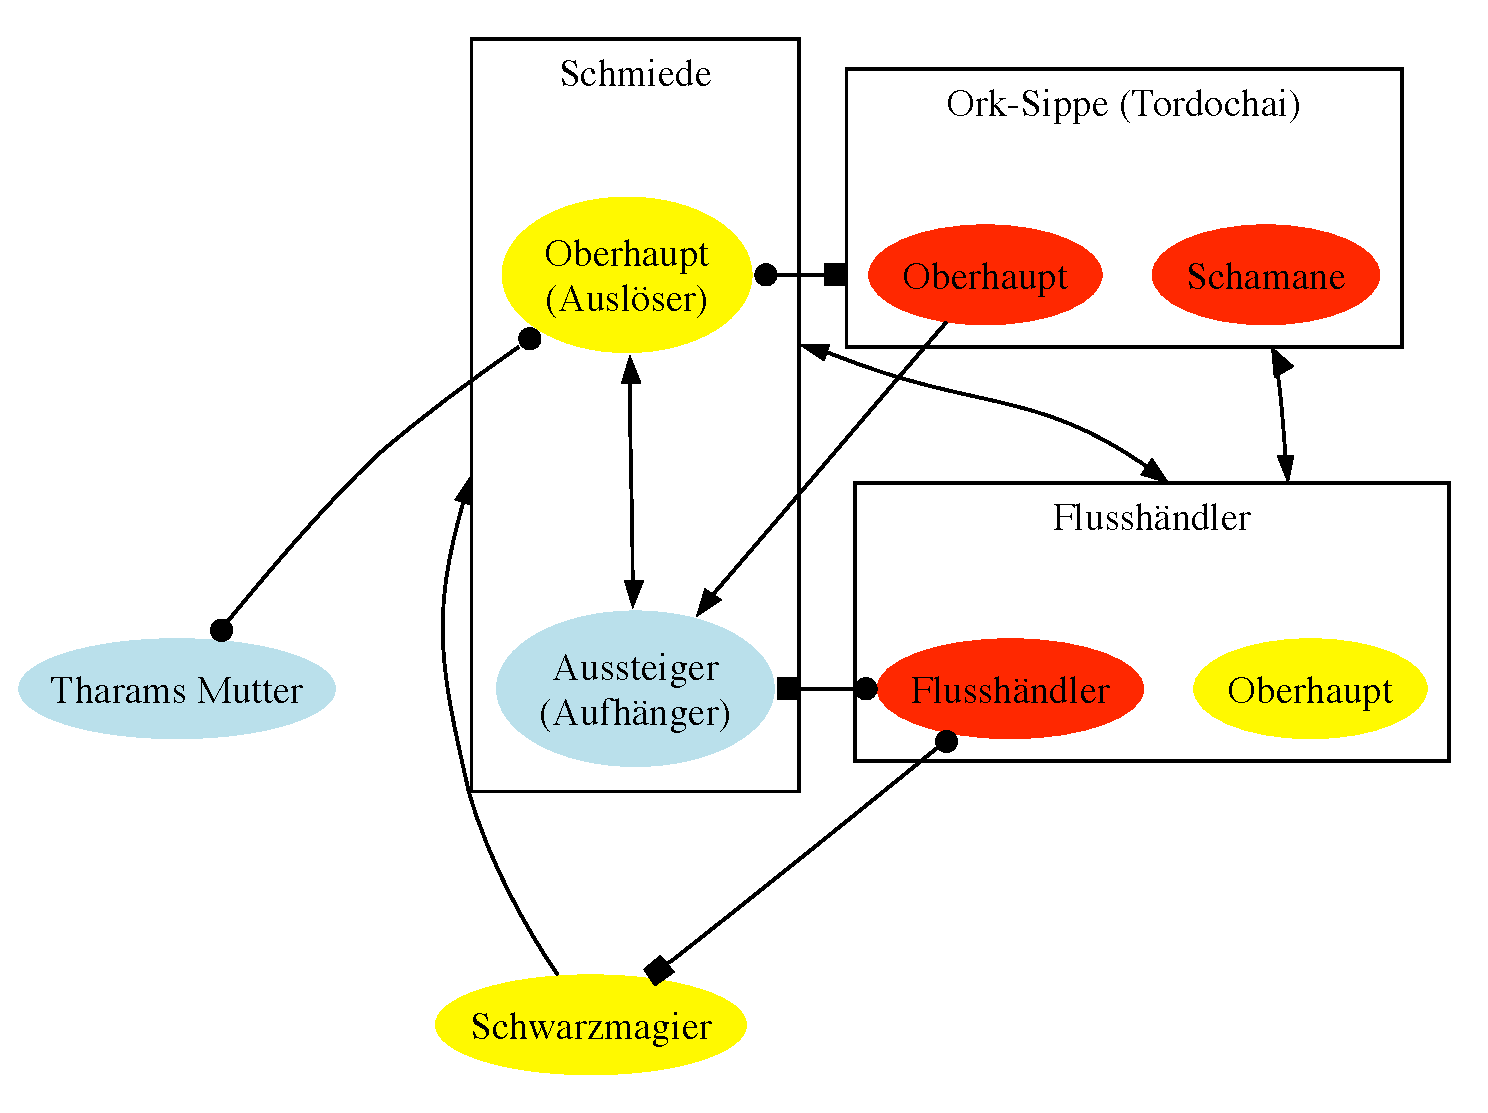
\includegraphics[width=0.95\textwidth]{pics/web2}}
\label{ABBKonfliktNetzBeispiel}
\hrule
\end{figure}

Insgesamt etwas lose angebunden ist vielleicht noch Ziliane. Jedoch durch ihre enge Anbindung an die Gruppe (immerhin die zweitwichtigste Person) und viele M"oglichkeiten zu Verhandlungen kann dieser Eindruck aber t"auschen.



\subsection{Beziehung zu den SCs}
In diesem Schritt werden die SLCs weiter ausgearbeitet. F"ur jeden SLC wird eine Motivation bzw. ein pers"onliches Ziel festgelegt und es wird gesagt, wie der SLC diese Ziele durchsetzen will, wenn die SCs auftreten: Versucht er ihre Hilfe in Anspruch zu nehmen, will er seine Ziele gegen die SCs durchsetzen oder versucht er, sie f"ur seine Zwecke auszunutzen?

Dazu werden dann noch Charakterz"uge festgelgt und sogenannte Handlungsgrenzen: Wie weit geht der SLC? Ist er eher vorsichtig oder geht er "uber Leichen? Als letztes werden noch die Flaggen notiert, die der SLC anspricht. Damit kann dann der SL die Geschichte so steuern, dass alle SCs gleicherma"sen angesprochen werden.

\begin{description}
  \item[Oberster Schmied:] M"ochte die eigene Macht st"arken und gleichzeitig den Handel zwischen Flussh"andlern und Finsterzwergen bek"ampfen. Hat R"uckhalt in seiner Gilde, dieser schwindet jedoch. Hat den Schwarzmagier bemerkt, wei"s aber nicht genau, von wem der kommt. Will SCs ausnutzen. Ist neidisch und reagiert leicht "uber. Geht im Extremfall "uber Leichen und bezahlt die Orks auch daf"ur.

  Flaggen: Ehrlichkeit von Tharam, Pazifismus von Bodowius, Selbstlosigkeit von Denidara

  \item[Aussteiger:] M"ochte Mord und Todschlag verhindern. Sucht Hilfe bei den SCs. Ist verzweifelt. Greift im Extremfall den Obersten Schmied offen verzweifelt an, um Tote durch die Orks zu verhindern.

  Flaggen: Pazifismus von Bodowius, Selbstlosigkeit von Denidara

  \item[Oberster Flussh"andler:] M"ochte seine Stellung ausbauen und beweisen, dass hinter den Orks die Schmiede stecken. M"ochte die SCs benutzen. Unmoralisch. Er ist bereit, gro"se Mengen Geld zu zahlen, um seine Ziele durchzusetzen.

  Flaggen: Ziliane Verhandlung und Klauen

  \item[Flussh"andler:] M"ochte den obersten Flussh"andler absetzen und selber an die Spitze. Nutzt den Aussteiger und den Schwarzmagier, um seine Position zu st"arken. Sieht in den SCs Feinde, die seinen Aufstieg verhindern k"onnten. Verheimlicht den Schwarzmagier und ist neidisch auf den obersten Flussh"andler. W"urde auch den Schwarzmagier gegen den obersten Flussh"andler oder seinen Schmiede-`Freund' einsetzen. Bei den SCs appelliert er an ihren Gerechtigkeitssinn.

  Flaggen: Selbstlosigkeit von Denidara

  \item[Ork-Bandenf"uhrer:] Wird durch das Geld der Schmiede motiviert. Gegner der SCs. F"uhrt brutal und fanatisch die Befehle vom obersten Schmied aus. F"uhlt sich "uberlegen und w"urde sich auch auf ein Duell mit Bodowius einlassen.

  Flaggen: Tharam Duell, Bodowius Pazifismus, Denidara Elfin

  \item[Ork-Schamane:] Sieht die Chance gekommen, dass er den Clan durch Spionaget"atigkeiten und Schl"age gegen Weiden unter den Orks nach vorne bringt. Gegner der SCs. Skrupellos, aber "uberlegt. Erkennt die SCs schnell als gef"ahrliche Gegner und geht gegen sie vor, kann sich aber nicht als Anf"uhrer aufspielen.

  Flaggen: 

  \item[Schwarzmagier:] Sieht seine Chance gekommen, "uber die H"andler die Politik von Trallop zu infiltrieren. Er nimmt den Flussh"andlern nicht wirklich ernst. M"ochte die SCs benutzen und macht daf"ur den SCs Angebote "uber magische Gegenst"ande. Er ist unmoralisch und verheimlicht den SCs gegen"uber die Verbindung zu den Flussh"andlern.

  Flaggen: Ziliane Verhandlungen, Bodowius schwarze Magie

  \item[Tharams Mutter:] Ist selber ungl"ucklich, dass sie ihre Stellung so ausgenutzt hat. Sie m"ochte die Situation aber nicht noch schlechter machen, daher versucht sie, ihren Missgriff zu verheimlichen. Wenn sie von selbst auf die Charaktere zugeht, dann braucht sie Hilfe, da ihre Verfehlung kurz vor der Aufdeckung steht.

  Flaggen: Tharam Bang
\end{description}



\subsection{Das Abenteuer}
Alleine aufgrund dieses Konflikt-Netzes kann sicherlich ein umfangreiches Abenteuer zusammengestellt werden, dass mit dem Schmied auf der Flucht beginnt, die Charaktere dann zu den Orks f"uhrt, von da k"onnten sie die Spur zu den Schmieden verfolgen und geraten dann in den Streit zwischen Flussh"andlern und Schmieden. Das ganze m"undet dann darin, dass Tharams von der Verfehlung seiner Mutter erf"ahrt und die Spieler entscheiden m"ussen, auf welche Seite sie sich stellen. Ein solches Abenteuer w"urde sicherlich einige Spielabende in Anspruch nehmen.

Soll aber das Konflikt-Netz f"ur den Auftakt einer Kampagne dienen, so sucht der SL zun"achst ein Zwischenziel. In diesem Beispiel soll es das Aufdecken der Machenschaften des Flussh"andlers sein, der den Schwarzmagier angeheuert hat und den Ausl"oser ausnutzt. Dar"uber sollen die SCs dann tiefer in den Sumpf blicken k"onnen. Das ganze Abenteuer soll als Einsteiger-Abenteuer konzipiert werden (sowohl f"ur die Chrakterspieler als auch f"ur den Spielleiter), daher wir es eine recht geradlinige und "ubersichtliche Story geben.

Daraus ergeben sich folgende drei Akte:
\begin{enumerate}
  \item Einleitung. Beginn mit einem Knaller: Kampf gegen die Orks. Der hat zwei m"ogliche Ausg"ange: Die Charaktere schaffen es, den Aussteiger zu retten oder der Aussteiger stirbt dabei. Egal wie, die Charaktere m"ussen einen Hinweis auf das Schmiede-Oberhaupt.

  \item Mittelteil. Die Charaktere sp"uren den Oberschmied auf. Der wiederum behauptet, dass der Schwarzmagier hinter der ganzen Sache steckt; er appelliert an das gute Gewissen der Helden. "Uber diesen finden sie dann den Flussh"andler, der den Schwarzmagier beauftragt hat.

  \item Ende. Die Charaktere werden mit dem Flussh"andler konfrontiert. Dieser hetzt den Schwarzmagier auf sie und erweist sich auch selber als unerwartet schlagkr"aftig.
\end{enumerate}



